\documentclass{article}

\def\ParSkip{} 
\input{../../common/ryantibs}
\usepackage[normalem]{ulem}
\usepackage{animate}

\title{Calibration and Forecast Scoring \\ \smallskip
\large Advanced Topics in Statistical Learning, Spring 2023 \\ \smallskip
Ryan Tibshirani }
\date{}

\begin{document}
\maketitle
\RaggedRight
\vspace{-50pt}

\section{Introduction}

In this lecture, we cover a topic that sits adjacent to conformal prediction in
a sense, which is calibration. We will cover the perspective(s) on calibration 
from the forecasting literature, where it is arguably the most developed. 
Instead of focusing solely on calibration, we'll cover some of the broader
theory of forecasting, pertaining to scoring rules, calibration, and ensembles.     

There is a rich literature on forecast scoring and calibration. This literature
has roots in statistics, but over the years it has been expanded and driven by
applied forecasting disciplines, primarily weather forecasting. It is still
quite an active area in terms of development: new results that seem foundational
in nature are still being discovered year to year.  

As per our usual comment, what we cover in this lecture is only a sample of what
is known in the theory of forecasting. Unlike other topics, we are not aware of
a book that gives a modern and comprehensive treatment of forecast scoring
rules, calibration, and so on. (Perhaps this would be premature, as these topics
are still in active development, and such a book will come later.) One of the
most active and influential researchers in forecasting theory today is Tilmann
Gneiting, and much of what we cover will be drawing from his work with
collaborators, such as \citet{gneiting2007strictly, gneiting2007probabilistic,
    ranjan2010combining, gneiting2013combining}.

\subsection{Probabilistic forecasting}

Our setup in this lecture will be that of \emph{probabilistic} (as opposed to
\emph{point}) forecasting. In this setting, a forecaster outputs a predicted
distribution $P$ of a given target $Y$ of interest. We will generally focus on
the case in which $Y$ is real-valued.

In probabilistic forecasting, both $P$ and $Y$ are random variables. To help
give context, we can think of an underlying sequential problem indexed by time
$t=1,2,3,\dots$, where:
\[
\text{a forecaster predicts $P_t$ for the distribution of $Y_t$, based on
  information available at times $s<t$}.
\]
Sometimes it will be more convenient to make the time dependence explicit in the
notation, but often it will be more convenient to hide it. 

\subsection{Probabilities or quantiles?}

It is most common to represent a probabilistic forecast $P$ by its cumulative
distribution function (CDF) $F$. Of course, instead of representing $P$ by its
CDF $F$, we can choose to represent it by its quantile function
$F^{-1}$. To be clear, the quantile function $F^{-1}$ is always well-defined,
even when $F$ is not continuous, and it is defined precisely as
\[
F^{-1}(t) = \inf\{ x : F(x) \geq t\}.
\]
When $F$ is not continuous, this shares some but not all properties of the 
usual inverse; recall the properties you derived on the homework.

An important note: typically these objects, the CDF $F$ or quantile function
$F^{-1}$, will be discretized in practice, and \emph{converting from one to the
  other will not always be possible/practical, particularly in the tails}. Thus
whether we choose at the outset to represent a predicted distribution by a CDF
or quantile function can have nontrivial implications on what tools we have at
our disposal for downstream tasks, like evaluation and aggregation.

Later, in Section \ref{sec:prob_quant}, we will discuss the differences between
aggregating probabilities (CDFs) and aggregating quantiles, in detail. Here, we
provide some higher-level practical considerations to keep in mind when choosing
to represent forecasts via probabilities versus quantiles.  

\begin{itemize}
\item A quantile representation for forecasts alleviates concerns about choosing
  the ``right'' bins for probability forecasts. Choosing bins in practice can be
  highly nonobvious, both in terms of the ``right''  scale, and the ``right''
  range.  

\item Quantiles can be directly fit a straightforward way, via quantile
  regression, and this can be carried out jointly over multiple probability
  levels. Constructing flexible (conditional) probability distributions can
  often be a more complex modeling task.  

\item For a discrete response that is concentrated around low values (such as 
  counts), a quantile representation may be undesirable since ``exact''
  quantiles only exist at a coarse set of probability levels (e.g., a reported
  level 0.05 quantile may actually be a level 0.09 quantile).     
\end{itemize}

\section{Scoring rules}

We now turn to discussing scoring rules, for evaluating probabilistic
forecasts. A \emph{scoring rule} (or simply a score) is a function $S$ that maps
a predicted distribution $P$ and target value $y$ to a real or infinite number 
\smash{$S(P, y) \in \widebar\R$} (where \smash{$\widebar\R = \R \cup \{\pm 
  \infty\}$} denotes the extended reals). We will, by convention, always take
the score to be negatively-oriented: a lower value means a better forecast.    

We use the notation $S(P, Q)$ to denote the expectation of the score over draws
$Y \sim Q$,  
\[
S(P, Q) = \E_{Y \sim Q} [S(P, Q)] = \int S(P, y) \, dQ(y).
\]

\subsection{Proper scores}

A scoring rule $S$ is said to be \emph{proper} if
\begin{equation}
\label{eq:proper}
S(P, Q) \geq S(Q, Q), \quad \text{for all $P,Q$},
\end{equation}
and \emph{strictly proper} if strict inequality holds in \eqref{eq:proper} for
$P \not= Q$. To quote \citet{gneiting2007strictly}, when $Q$ denotes the 
distribution of $Y$ and the score $S$ is proper: ``the forecaster has no
incentive to predict any $P \not= Q$ and is encouraged to report his or her true
belief''.  

Several examples of proper scores are given below. (An example of an intuitively
appealing but improper score will also be given.) Throughout, we will flexibly
write the scores as taking densities, CDFs, or quantile functions as inputs
(instead of distributions), as convenient.        

\paragraph{Log score.}

\def\KL{\mathrm{KL}}

For a forecast that has density or probability mass function $p$, \emph{log
  score} is defined by 
\begin{equation}
\label{eq:logs}
\mathrm{LogS}(p, y) = -\log p(y).
\end{equation}
This is a strictly proper score. To see this, we compute:
\begin{equation}
\label{eq:kl_div}
\mathrm{LogS}(p, q) - \mathrm{LogS}(q, q) = \int \log \frac{q(y)}{p(y)} q(y) \, 
dy,
\end{equation}
which recall is the Kullback-Leibler (KL) divergence between $q$ and $p$, often
denoted $\KL(q,p)$ (note carefully the order of arguments here). This is known
to be nonnegative, and positive for $p \not= q$.

Log score \eqref{eq:logs} very sharply penalizes forecasts that place
insufficiently low probability on events that materialize: for small $p(y)$, the
score $-\log p(y)$ is very large (and asymptotes at $p(y) = 0$).  

\paragraph{Interlude: connection to Bergman divergence.}

KL divergence is a special instance of a \emph{Bregman divergence}, which is of
the form (note carefully the order of arguments)
\begin{equation}
\label{eq:bregman}
d_\phi(q,p) = \phi(q) - \phi(p) - \langle D\phi(p), q - p \rangle,
\end{equation}
for a convex differentiable function $\phi$, with derivative $D\phi$, and
suitable inner product $\langle \cdot, \cdot \rangle$. In particular, KL
divergence \eqref{eq:kl_div} is a Bregman divergence \eqref{eq:bregman} when
$\phi(p) = \int p(y) \log p(y) \, dy$, and $\langle p, q \rangle = \int p(y)
q(y) \, dy$.   

The connection between log score and Bregman divergence is no coincidence, and
the connection between proper scores and Bregman divergences runs much
deeper. If $\phi$ is strictly convex, then by the first-order characterization
for convexity, we have $d_\phi(q,p) \geq 0$, with strict inequality for $p \not= 
q$. Due to this fact, if $S$ is any score for which we have the Bregman
representation (for strictly convex $\phi$)   
\begin{equation}
\label{eq:bregman_rep}
S(p, q) - S(q, q) = d_\phi(q, p),
\end{equation}
then $S$ is strictly proper. In essence, the converse is true as well. The
formal details will be covered in Section \ref{sec:bregman_rep}. 

\paragraph{Quadratic score.}

For a forecast that has density or probability mass function $p$,
\emph{quadratic} or \emph{Brier score} is defined by   
\begin{equation}
\label{eq:quads}
\mathrm{QuadS}(p, y) = 2p(y) - \|p\|_2^2,
\end{equation}
where $\|p\|_2^2 = \int p(y)^2 \, dy$. This is a strictly proper score. To see
this, we compute:  
\[
S(p, q) - S(q, q) = \|p\|_2^2 - 2 \int p(y) q(y) \, dy + \|q\|_2^2 =
\|p-q\|_2^2,
\]
which is the $L^2$ distance between $p$ and $q$. It is nonnegative, and
positive for $p \not= q$.  

Quadratic score \eqref{eq:quads} is more robust than log score \eqref{eq:logs},
in the sense that it is gentler in penalizing forecasts that place low
probability on events that materialize.  

\paragraph{Linear score.}

For a forecast that has density or probability mass function $p$,
\emph{linear score} is defined by   
\[
\mathrm{LinS}(p, y) = -p(y).
\]
We mention this score because it may seem intuitively appealing, but is
\emph{not proper} (and is basically never used in practice). To see this, let
$q$ be the standard normal density, and let $p$ be the uniform density on the 
interval $(-\epsilon, \epsilon)$, for some $\epsilon>0$ to be specified
later. Then    
\begin{align*}
\mathrm{LinS}(p, q) - \mathrm{LinS}(q, q) 
&= \int q(y)^2 \, dy - \frac{1}{2\epsilon} 
  \int_{-\epsilon}^\epsilon q(y) \, dy \\
&= \frac{1}{2\pi} \int e^{-y^2} \, dy -  \frac{1}{\sqrt{2\pi}}
  \frac{1}{2\epsilon} \int_{-\epsilon}^\epsilon e^{-y^2/2} \, dy \\   
&= \frac{1}{\sqrt{2\pi}} \bigg( 1/\sqrt{2} - \frac{1}{2\epsilon}
\int_{-\epsilon}^\epsilon e^{-y^2/2} \, dy \bigg).
\end{align*}
The last display will be negative for small enough $\epsilon > 0$: in 
particular, for \smash{$\epsilon < \sqrt{\log 2}$}, the integrand in the above
satisfies \smash{$e^{-y^2/2} > 1/\sqrt{2}$}, so the integral satisfies
\smash{$\frac{1}{2\epsilon}  \int_{-\epsilon}^\epsilon e^{-y^2/2} \, dy > 
  1/\sqrt{2}$}.

\paragraph{Continuous ranked probability score.}

Not all probabilistic forecasts can be expressed in terms of a density or
probability mass function. For example, some forecast distributions might place
a point mass at zero, and would be otherwise continuous. The \emph{continuous
  ranked probability score} (CRPS) accommodates this and, in general, any
forecast expressed in terms of a predicted CDF $F$. It is defined by 
\begin{equation}
\label{eq:crps}
\mathrm{CRPS}(F, y) = \int (F(x) - 1\{y \leq x\})^2 \, dx. 
\end{equation}
This is a strictly proper score. To see this, we compute: 
\begin{align*}
\mathrm{CRPS}(F, G) - \mathrm{CRPS}(G ,G) 
&= \int \Big( F(x)^2 - G(x)^2 - 2(F(x) - G(x)) \E_{Y \sim G}[ 1\{Y \leq x\} ]
  \Big) \, dx \\
&= \int \Big( F(x)^2 - G(x)^2 - 2(F(x) - G(x)) G(x) \Big) \, dx \\
&= \int (F(x) - G(x))^2 \, dx.
\end{align*}
This is the Cram{\'e}r-von Mises distance between $F$ and $G$. It is
nonnegative, and positive for $p \not= q$.   

CRPS \eqref{eq:crps} has become recently quite popular in various applied
forecasting communities (e.g., in meterological sciences), in part because it is
considered more robust than log score, and as already mentioned, it is more
broadly applicable, beyond log \eqref{eq:logs} and quadratic \eqref{eq:quads}
scores. However, unlike the latter two, CRPS is nontrivial to compute. Some
authors have pursued quadrature-based approximations to the integral defining
CRPS. A simpler approximation is given by noting its connection to weighted
interval score/quantile loss, which will be covered just a bit later on.

\paragraph{Interval score.}

For an interval forecast expressed as $[\ell_\alpha, u_\alpha]$, where the lower
and upper endpoints $\ell_\alpha = F^{-1}(\alpha/2)$ and $u_\alpha =
F^{-1}(1-\alpha/2)$ are the predicted $\alpha/2$ and $1-\alpha/2$ quantiles of
the forecast distribution, \emph{interval score} is defined by 
\[
\mathrm{IS}_\alpha( [\ell_\alpha, u_\alpha], y) = 
(u_\alpha - \ell_\alpha) + \frac{2}{\alpha} \cdot
\mathrm{dist}(y, [\ell_\alpha, u_\alpha])
\]
where \smash{$\mathrm{dist}(y, S) = \inf_{x \in S} |x-y|$} for a set $S$. We can
see that this combines a reward for sharpness (first term) and a penalty for 
miscoverage (second term). For a collection of interval forecasts
$[\ell_\alpha, u_\alpha]$, $\alpha \in \cA$, \emph{weighted interval score}
(WIS) is defined by
\begin{align}
\nonumber
\mathrm{WIS}_\cA \big( \{[\ell_\alpha, u_\alpha]\}_{\alpha \in \cA}, \, y \big)  
&= \sum_{\alpha \in \cA} \alpha \cdot \mathrm{IS}_\alpha( [\ell_\alpha,
  u_\alpha], y) \\
\label{eq:wis}
&=\sum_{\alpha \in \cA} \Big(\alpha (u_\alpha - \ell_\alpha) + 2 \cdot
  \mathrm{dist}(Y, [\ell_\alpha, u_\alpha]) \Big).
\end{align}
Weighted interval score (and thus interval score, as effectively a special case)
is a proper score for predicting the quantiles at levels $\alpha/2$ and
$1-\alpha/2$, over $\alpha \in \cA$. To be clear, here we say (by analogy to 
\eqref{eq:proper}) that a score $S$ defined in terms of a discrete set of
predicted quantiles \smash{$\{q_\tau\}_{\tau \in \cT}$} if it holds that   
\begin{equation}
\label{eq:proper_q}
S \big( \{q_\tau\}_{\tau \in \cT}, \, F \big) \geq S \big(
\{F^{-1}(\tau)\}_{\tau \in \cT}, \, F \big), \quad \text{for all
$\{q_\tau\}_{\tau \in \cT}$, and all $F$},    
\end{equation}
where as usual \smash{$S(\{q_\tau\}_{\tau \in \cT}, \, F) = \E_{Y \sim F}[
  S(\{q_\tau\}_{\tau \in \cT}, \, Y)]$}. Propriety of weighted interval score  
can be verified by drawing a connection to quantile loss, covered shortly.  

\paragraph{Quantile score.}

For a forecast expressed as a collection of predicted quantiles $q_\tau$, $\tau
\in \cT$, \emph{quantile score} (QS) is defined by 
\begin{equation}
\label{eq:qs}
\mathrm{QS}_\cT \big( \{q_\tau\}_{\tau \in \cT}, \, y \big) = 
\sum_{\tau \in \cT} \rho_\tau(y - q_\tau),
\end{equation}
where $\rho_\tau(u) = \tau |u|$ for $u \geq 0$ and $(1-\tau) |u|$ for $u < 0$,
often called the tilted $\ell_1$ loss at the level $\tau$. This is nothing else
than the loss that is the standard choice in \emph{quantile regression}. That
quantile score is proper, in the sense of \eqref{eq:proper_q}, follows from the
standard fact that the true level $\tau$ quantile is a minimizer of the expected
tilted $\ell_1$ loss at the level $\tau$.

\paragraph{Connection between WIS and QS.}

The following is an connection between WIS \eqref{eq:wis} and QS \eqref{eq:qs}: 
for any set $\cA$ of error levels, if we define a corresponding set
\smash{$\cT = \cup_{\alpha \in \cT} \, \{ \alpha/2, 1-\alpha/2 \}$} of
probability levels, then it holds that     
\begin{equation}
\label{eq:wis_qs}
\mathrm{WIS}_\cA \big( \{[\ell_\alpha, u_\alpha]\}_{\alpha \in \cA}, \, y \big)  
= 2 \cdot \mathrm{QS}_\cT \big( \{q_\tau\}_{\tau \in \cT}, \, y \big).
\end{equation}
The equivalence \eqref{eq:wis_qs} between WIS and QS can be verified by
straightforward algebra. Apart from being interesting, and lending a new 
interpretation to how quantile score \eqref{eq:qs} combines a sharpness reward
with a miscoverage penalty (recall the discussion following \eqref{eq:wis}), it
is also a useful observation as it provides an indirect but simple proof that
WIS \eqref{eq:wis} is proper, in the sense of \eqref{eq:proper_q}.

\paragraph{Connection between CRPS and QS.}

The connections continue: interestingly, CRPS \eqref{eq:crps} also has an
equivalent formulation in terms of QS: if $F$ differentiable, with density $f$,
and admits an expectation, $\int y f(x) \, dy < \infty$, then    
\begin{equation}
\label{eq:crps_qs}
\int (F(x) - 1\{y \leq x\})^2 \, dx = 
2 \int \rho_\tau(y - F^{-1}(\tau)) \, d\tau. 
\end{equation}
The right-hand side is an integral of QS all probability levels $\tau \in [0,1]$.
This is quite interesting because these two error metrics---CRPS and QS---are 
motivated from very different perspectives, not to mention different
parametrizations (CDF space versus quantile space).   

The equivalence in \eqref{eq:crps_qs} appears to have been discovered by
\citet{laio2007verification}; their argument uses integration by parts, but it
ignores a few subtleties, and so here we reproduce the proof from
\citet{fakoor2021flexible}, which basically just fills in a few missing details.
Starting with the right-hand side in \eqref{eq:crps_qs}, we can substitute 
$y=F^{-1}(\tau)$ to rewrite the integral as   
\[
2 \int (1\{y \leq F^{-1}(\tau)\} - \tau) (F^{-1}(\tau)-X) \, d\tau =  
2 \int (1\{y \leq x\} - F(x)) (x-y) f(x) \, dx.
\]
Let $u'(x)=2(1\{y \leq x\} - F(x)) f(x)$ and $v(x)=x-y$. The idea is now to use 
integration by parts, but there are two subtleties. First, one has to be careful 
about framing the antiderivative $u$ of $u'$, since $x \mapsto 1\{y \leq x\}$ is
not classically differentiable. Note that we can actually redefine $u'$ to be   
\[
u'(x) = 2(1\{y \leq x\} - F(x)) (f(x) - \delta_y(x)),
\]
where $\delta_y$ is the Dirac delta function centered at $y$, because the
``extra'' piece integrates to zero:   
\[
\int 2(1\{y \leq x\} - F(x)) (x-y) \delta_y(x) \, dx =  
2(1\{y \leq x\} - F(x)) (x-y) \Big|_{x=y} = 0. 
\]
With this new definition of $u'$, its antiderivative is rigorously
\[
u(x) = -(1\{y \leq x\} - F(x))^2,
\] 
because, in the distributional sense, the derivative of the heavyside function
$x \mapsto 1\{y \leq x\}$ is indeed the delta function $\delta_y$. Thus we have   
\begin{align*}
\int u'(x) v(x) \, dx
&= u(x) v(x) \Big|_{-\infty}^\infty - \int u(x) v'(x) \,  dx \\ 
&= -(1\{y \leq x\} - F(x))^2 (x-y) \Big|_{-\infty}^\infty + 
\int (1\{y \leq x\} - F(x))^2 \, dx. 
\end{align*}
The second subtlety is to show that the first term above is indeed zero.  
This is really a question of how fast the tails of $F$ decay. As $F$ yields an
expectation, note that we must have $1-F(x) \lesssim x^{-p}$ for $p>1$ (since
$1/x$ is not integrable on any one-sided interval $[q,\infty)$ for $q>0$). Hence   
\[
(1-F(x)) x \lesssim x^{-p+1} \to 1 \quad \text{as $x \to \infty$},
\]
and the other limit, as $x \to -\infty$, is similar.

\paragraph{Quick recap.}

Here is a quick recap of what we learned on our tour of scores. Log score
\eqref{eq:logs} and quadratic score \eqref{eq:quads} are classical choices, each
strictly proper, with the former being more aggressive at penalizing
underconfidence assigned to rare events. CRPS \eqref{eq:crps} is a more modern
alternative, also strictly proper, which has become popular due to its
robustness and generality, but is nontrivial to compute.        

For forecasts specified in terms of quantiles at discrete probability levels,
WIS \eqref{eq:wis} and QS \eqref{eq:qs} are each proper, simple, and popular
choices, motivated from different perspectives; and in fact they turn out to be 
equivalent \eqref{eq:wis_qs}. Moreover, CRPS turns out to be equivalent
to an integrated quantile score \eqref{eq:crps_qs} over all probability
levels. Thus a simple approximation to CRPS in practice would be to discretize
at any desired set of probability levels and use this to define WIS/QS;
propriety is always maintained, in the sense of \eqref{eq:proper_q}, for any
choice of discretization.     

Figures \ref{fig:scores1} and \ref{fig:scores2} visualize some of these scores
in action. 

\begin{figure}[p]
\centering
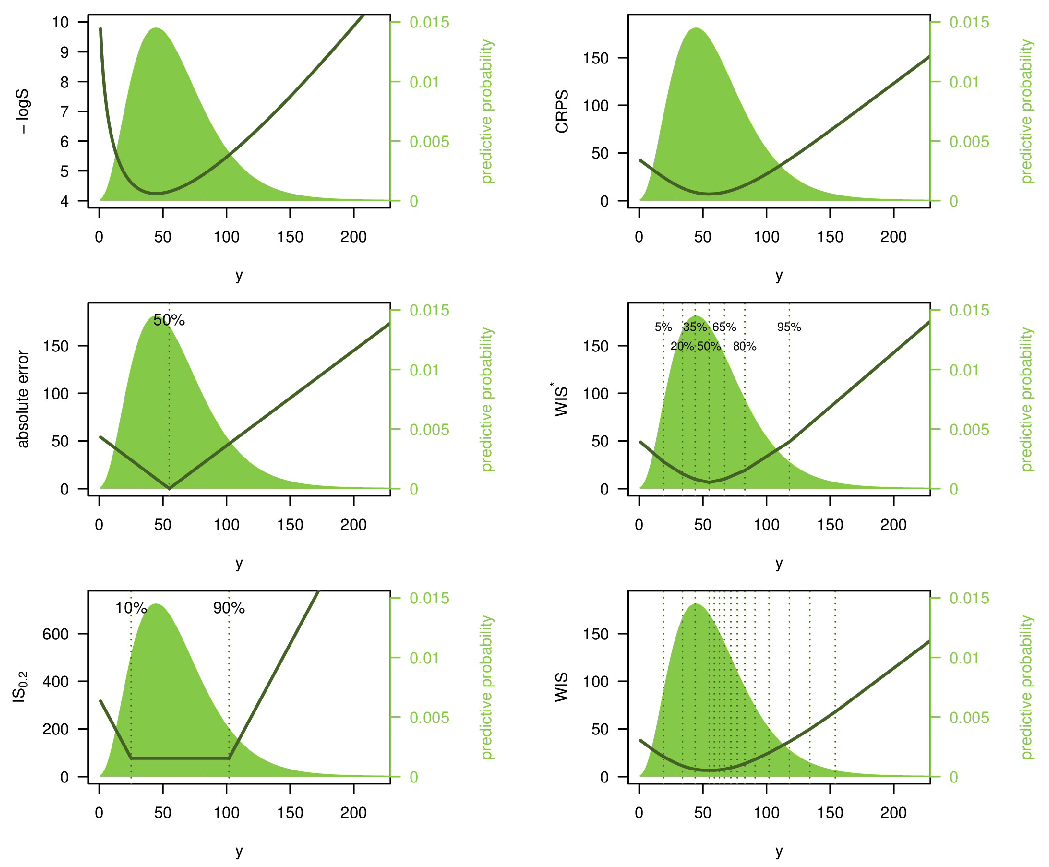
\includegraphics[width=0.975\textwidth]{scores1.png}
\caption{\it Various scores visualized as functions of $y$, based on the
  predicted distribution plotted in green. Here WIS$^*$ and WIS denote two
  versions of weighted interval score at a coarser and finer set of probability
  levels, respectively. Credit: \citet{bracher2021evaluating}.}       
\label{fig:scores1}   

\bigskip\medskip

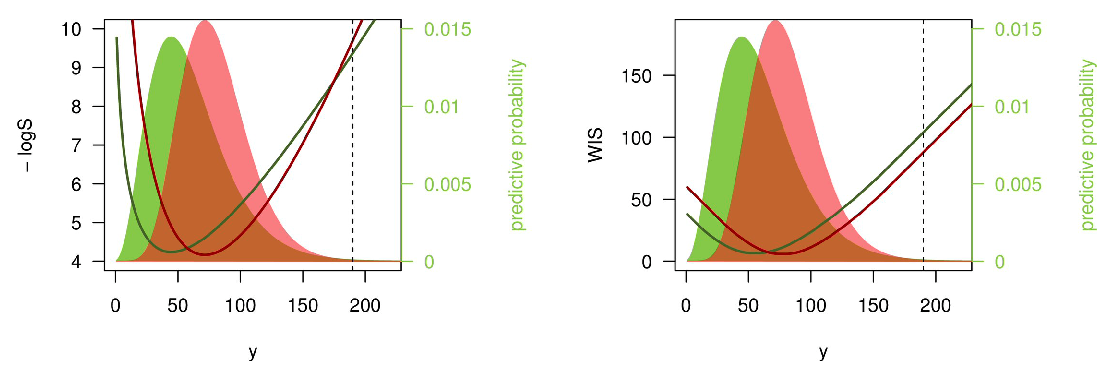
\includegraphics[width=0.975\textwidth]{scores2.png}
\caption{\it Comparison between log score and WIS for two predicted
  distributions: $P$ in green and $Q$ in red. Note that $G$ has a higher
  expectation, while $F$ is more dispersed. If we consider an event $y$ that is
  marked as a dashed vertical line, then we see log score prefers $F$ to $G$,
  while WIS prefers $G$ to $F$. Credit: \citet{bracher2021evaluating}.}           
\label{fig:scores2}
\end{figure}

\subsection{Bregman representation}
\label{sec:bregman_rep}

Below we state an important result from \citet{gneiting2007strictly} that shows
that the Bregman representation \eqref{eq:bregman_rep} which we saw was possible 
for log score (and quadratic score, and CRPS) is ``no accident'', and in a
precise sense, characterizes \emph{all} proper scores.    

Before stating the result, we must introduce some terminology and
concepts. Recall that by convention, we take all scores to be
negatively-oriented. First, we say a score $S$ is \emph{regular} if $S(P,P)$ is 
real-valued for all $P$ (i.e., we allow $S(P, Q) = \infty$ for $P \not=
Q$). Regularity is essentially needed in order for subderivatives (defined 
shortly) to make sense but we omit the details. 

Next, we refine the definition of propriety: for a class $\cP$ of probability
distributions, we say a score $S$ is \emph{proper relative to $\cP$} if
\eqref{eq:proper} holds for $P,Q \in \cP$, with \emph{strictly proper relative 
  to $\cP$} again meaning that the inequality is strict for $P \not= Q$.  

Lastly, for a function $\phi$ acting over a set of distributions $\cP$, with
each $P \in \cP$ having a sample space $\cY$, we say that $D\phi(P, \cdot)$ is a
\emph{subderivative} of $\phi$ at $P \in \cP$ provided that 
\begin{equation}
\label{eq:subderiv}
\phi(Q) \geq \phi(P) + \int D\phi(P, y) \, d(Q-P)(y), \quad \text{for all $Q \in
  \cP$}.  
\end{equation}

We are now ready to state the result. 

\begin{theorem}
Let $\phi$ be convex function acting over a set of distributions $\cP$. Define
for $P \in \cP$ and $y \in \cY$ the regular score  
\begin{equation}
\label{eq:phi_score}
S(P, y) = -\phi(P) - D\phi(P, y) + \int D\phi(P, y) \, dP(y),
\end{equation}
where $D\phi(P, \cdot)$ is a subderivative of $\phi$ at $P$. Then for any $P,Q
\in \cP$, 
\begin{equation}
\label{eq:phi_div}
S(P, Q) - S(Q, Q) = \underbrace{\phi(Q) - \phi(P) - \int D\phi(P, y) \,
  d(Q-P)(y)}_{d_\phi(Q,P)},
\end{equation}
which is the Bregman divergence with respect to $\phi$, and the score $S$ is
proper relative to $\cP$.  

Conversely, if $S$ is a regular score that is proper relative to $\cP$, then $S$
can be written in the form \eqref{eq:phi_score} with respect to the convex
function $\phi(P) = -S(P, P)$, and the Bregman representation \eqref{eq:phi_div}
holds.    

Finally, the above equivalence also holds when the terms convex and proper are
replaced by strictly convex and strictly proper, respectively.  
\end{theorem}

\begin{proof}
If $\phi$ is convex and we define $S$ according to \eqref{eq:phi_score}, then
\eqref{eq:phi_div} follows by direct algebra. Meanwhile, $d_\phi(Q, P) \geq 0$
for any $P,Q \in \cP$ by definition of the subderivative \eqref{eq:subderiv},
which proves that $S$ is proper relative to $\cP$. For the other direction, if
$S$ is regular and proper relative to $\cP$, then letting $\phi(Q) = -S(Q, Q)$
is equivalent to letting  
\[
\phi(Q) = -\inf_{P \in \cP} \, S(P, Q) = \sup_{P \in \cP} \, -S(P, Q).
\]
For fixed $P$, the function $Q \mapsto -S(P, Q)$ is linear, and hence convex,
and thus by the above $\phi$ is a pointwise supremum of convex functions and
hence itself convex. Furthermore, we can see that $D\phi(P, \cdot) = -S(P,
\cdot)$ is a valid subderivative of $\phi$, since \eqref{eq:subderiv} becomes 
$-S(Q, Q) \geq -S(P, Q)$ for all $Q \in \cP$, which is satisfied because $S$ is 
proper relative to $\cP$. Under the choice $D\phi(P, \cdot) = -S(P, \cdot)$, the 
score representation \eqref{eq:phi_score} is a tautology. The Bregman
representation \eqref{eq:phi_div} again follows by simple algebra. This
completes the proof of the claimed equivalence, and the arguments for the strict
version of the result follow similarly.
\end{proof}

Even though our focus has been (and will continue to be) real-valued forecasts,
it is worth emphasizing that the previous theorem treats the sample space $\cY$
as arbitrary. In the case of categorical forecasts, where $\cY = \{1,\dots,k\}$,
we get the following corollary, which is originally due to 
\citet{savage1971elicitation}. We denote the standard $k$-dimensional 
probability simplex by \smash{$\Delta^k = \{ p \in \R^k : p \geq 0, \;
  \sum_{i=1}^k p_i = 1\}$}.

\begin{corollary}
Let $\cY = \{1,\dots,k\}$. Then a regular score $S$, which we treat as acting on
a vector of probabilities $p \in \Delta^k$, is proper with respect to the set of
all distributions on $\{1,\dots,k\}$ if and only if 
\[
S(p, i) = -\phi(p) - D_i\phi(p) + \langle D\phi(p), p \rangle , \quad \text{for
  $i=1,\dots,k$},
\]
for a convex function $\phi$ on $\Delta^k$, where $D\phi(p)$ denotes the
subgradient of $\phi$ at $p$ (with components $D_i\phi(p)$, $i=1,\dots,k$). The
same equivalence also holds when the terms convex and proper are replaced by
strictly convex and strictly proper, respectively.     
\end{corollary}

\section{Modes of calibration}

Next we turn to calibration. There are in fact many modes or ``flavors'' of
calibration, and they are related but not all equivalent. We walk through three
such definitions, in the following subsections. But first, we recap some
important preliminary concepts, which will help give motivation for the
definitions.    

\subsection{Preliminary concepts}

\def\deq{\overset{d}{=}}

For any CDF $F$ (fixed or random) and target random variable $Y$, we define  
\begin{equation}
\label{eq:pit}
F^*(Y) = V \cdot F(Y) + (1-V) \cdot F(Y^-),
\end{equation}
where $V \sim \mathrm{Unif}(0,1)$ is independent of $F$ and $Y$, and
\smash{$F(y^-) = \lim_{x \to y^-} F(x)$}. This is called the \emph{probability
  integral transform} (PIT) associated with $F$ and $Y$. If $F$ is continuous
(i.e., if $F$ is a continuous function, and hence invertible) almost surely,
then the PIT reduces to $F^*(Y) = F(Y)$.    

Recall that if we take $F$ to be \emph{fixed} and equal to the CDF of $Y$, then
$F^*(Y)$ (or $F(Y)$ in the continuous case) is itself standard uniform. You
proved this fact on the homework fact. We can write this simply as   
\[
F^*(Y) \deq U,
\]
where here and throughout the remainder of these lecture notes section, we
denote $U$ to denote a standard uniform random variable, $U \sim
\mathrm{Unif}(0,1)$, independent of everything else that is random. Recall also
that of we take $F^{-1}$ to be \emph{fixed} and equal to the quantile function
of $Y$, then  
\[
F^{-1}(U) \deq Y,
\]
which you also proved on the homework. The definitions of probabilistic and
marginal calibration, covered over the next two subsections, are based on
requiring the above two properties to hold, respectively, in the case when $F$
is also random.   

\subsection{Probabilistic calibration}

A forecaster with predicted CDF $F$ is said to be \emph{probabilistically 
  calibrated} for a target $Y$ if 
\begin{equation}
\label{eq:prob_calib}
F^*(Y) \deq U
\end{equation}
where recall $F^*(Y)$ is defined as in \eqref{eq:pit}, and $U \sim 
\mathrm{Unif}(0,1)$. To be explicit, here both $F$ and $Y$ are
\emph{random}. Another name for probabilistic calibration is \emph{PIT
  calibration}, and another way of writing \eqref{eq:prob_calib} is  
\[
\P\Big( V \cdot F(Y) + (1-V) \cdot F(Y^-) \leq t \Big), \quad \text{for all $t
  \in [0,1]$}, 
\]
for $V \sim \mathrm{Unif}(0,1)$, independent of $F$ and $Y$, which is typically
how you will see it defined. 

\paragraph{Quantile reformulation.}

When $F$ is continuous almost surely, then we can reinterpret probabilistic
calibration as follows: $F$ is calibrated for $Y$ if   
\[
\P(Y \leq F^{-1}(t)) = t, \quad \text{for all $t \in [0,1]$}. 
\]
This is highly intuitive; for example, when we inspect the forecaster's
predicted quantile at the level 0.9, the target $Y$ should lie below this 90\% 
of the time, and so on, for all probability levels.   

\paragraph{Dispersion: over and under.}

If $F$ places too much mass in the tails, then the PIT $F^*(Y)$ will be
U-shaped, and its variance will be large compared to that of a uniform
distribution. Conversely, if $F$ places insufficient mass in the tails, then the 
PIT $F^*(Y)$ will be upside-down U-shaped, and its variance will be comparably
small. Recalling $U \sim \mathrm{Unif}(0,1)$ denotes a standard uniform random 
variable, this leads to the following definitions, in the context of PIT
calibration:   

\begin{itemize}
\item $F$ is said to be \emph{overdispersed} for $Y$ if $\Var[F^*(Y)] < \Var[U]$;
\item $F$ is said to be \emph{underdispersed} for $Y$ if $\Var[F^*(Y)] >
  \Var[U]$. 
\end{itemize}

Figures \ref{fig:pit1} and \ref{fig:pit2} provide examples.

\begin{figure}[p]
\centering
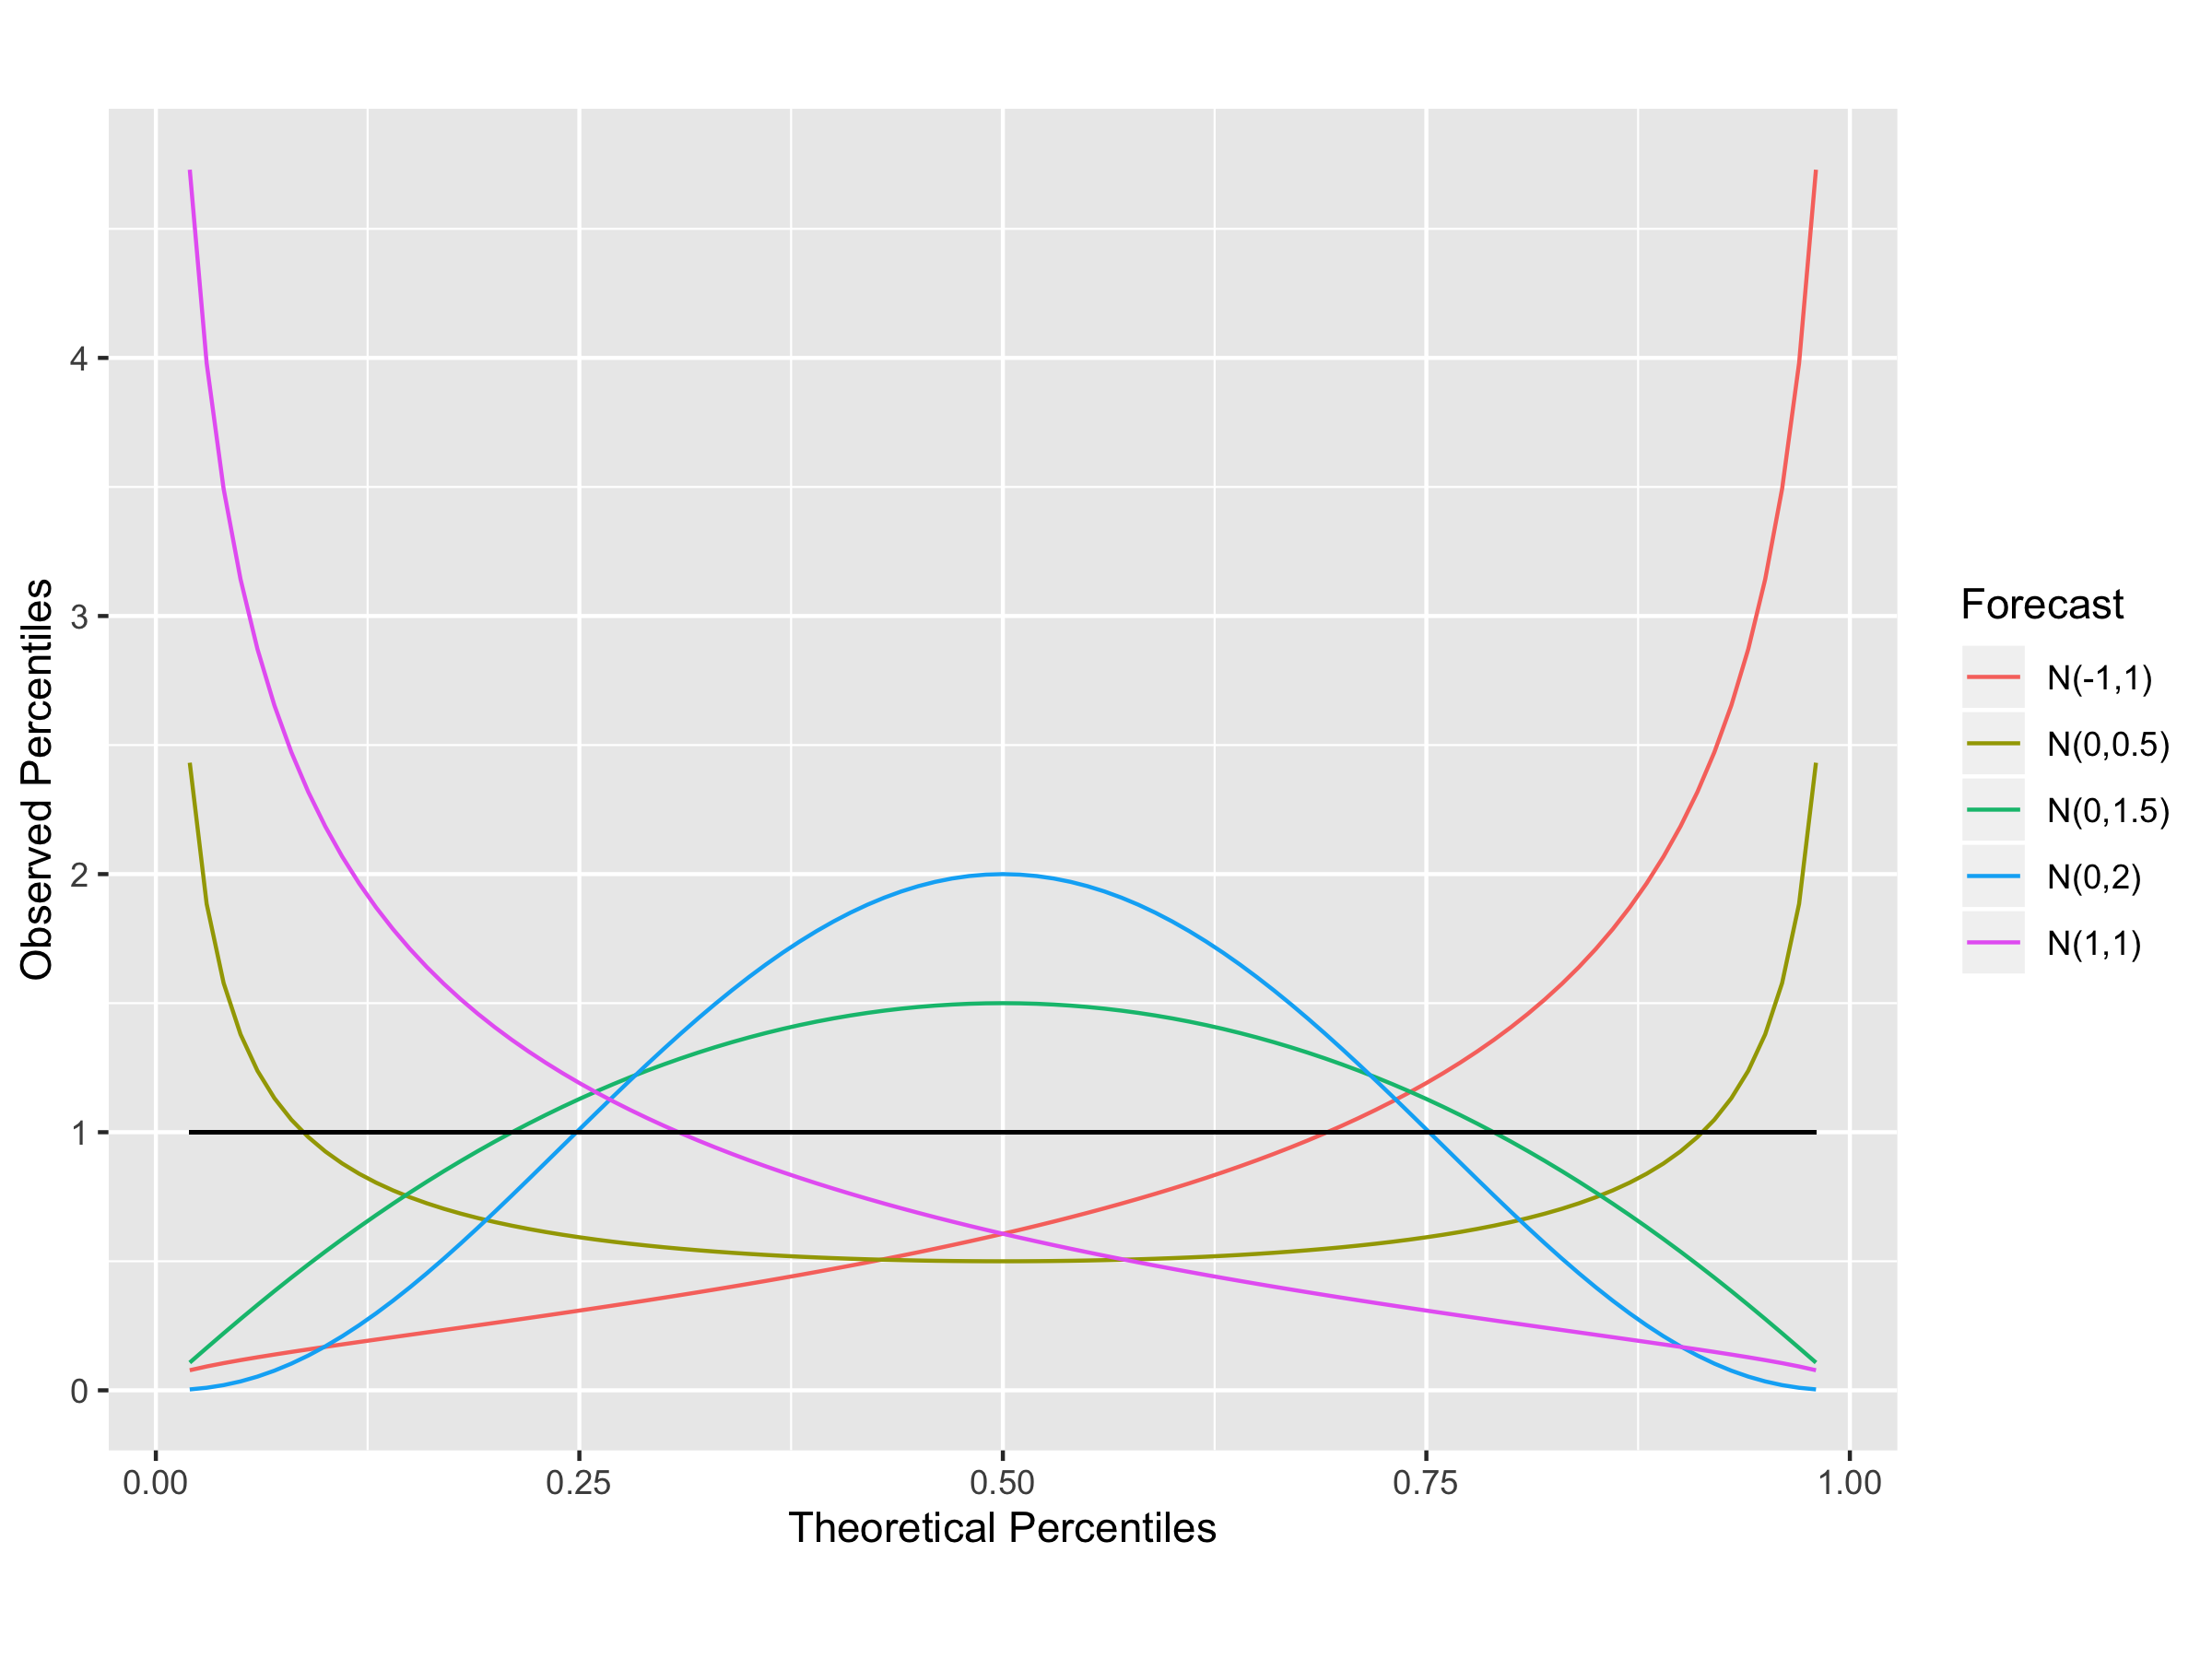
\includegraphics[width=0.7\textwidth]{pit1.png}
\vspace{-15pt}
\caption{\it Densities of PIT distributions for several simple normal
  forecasters, when the true target distribution is $N(0,1)$. Credit:
  \citet{rumack2022recalibrating}.}        
\label{fig:pit1}   

\bigskip\medskip

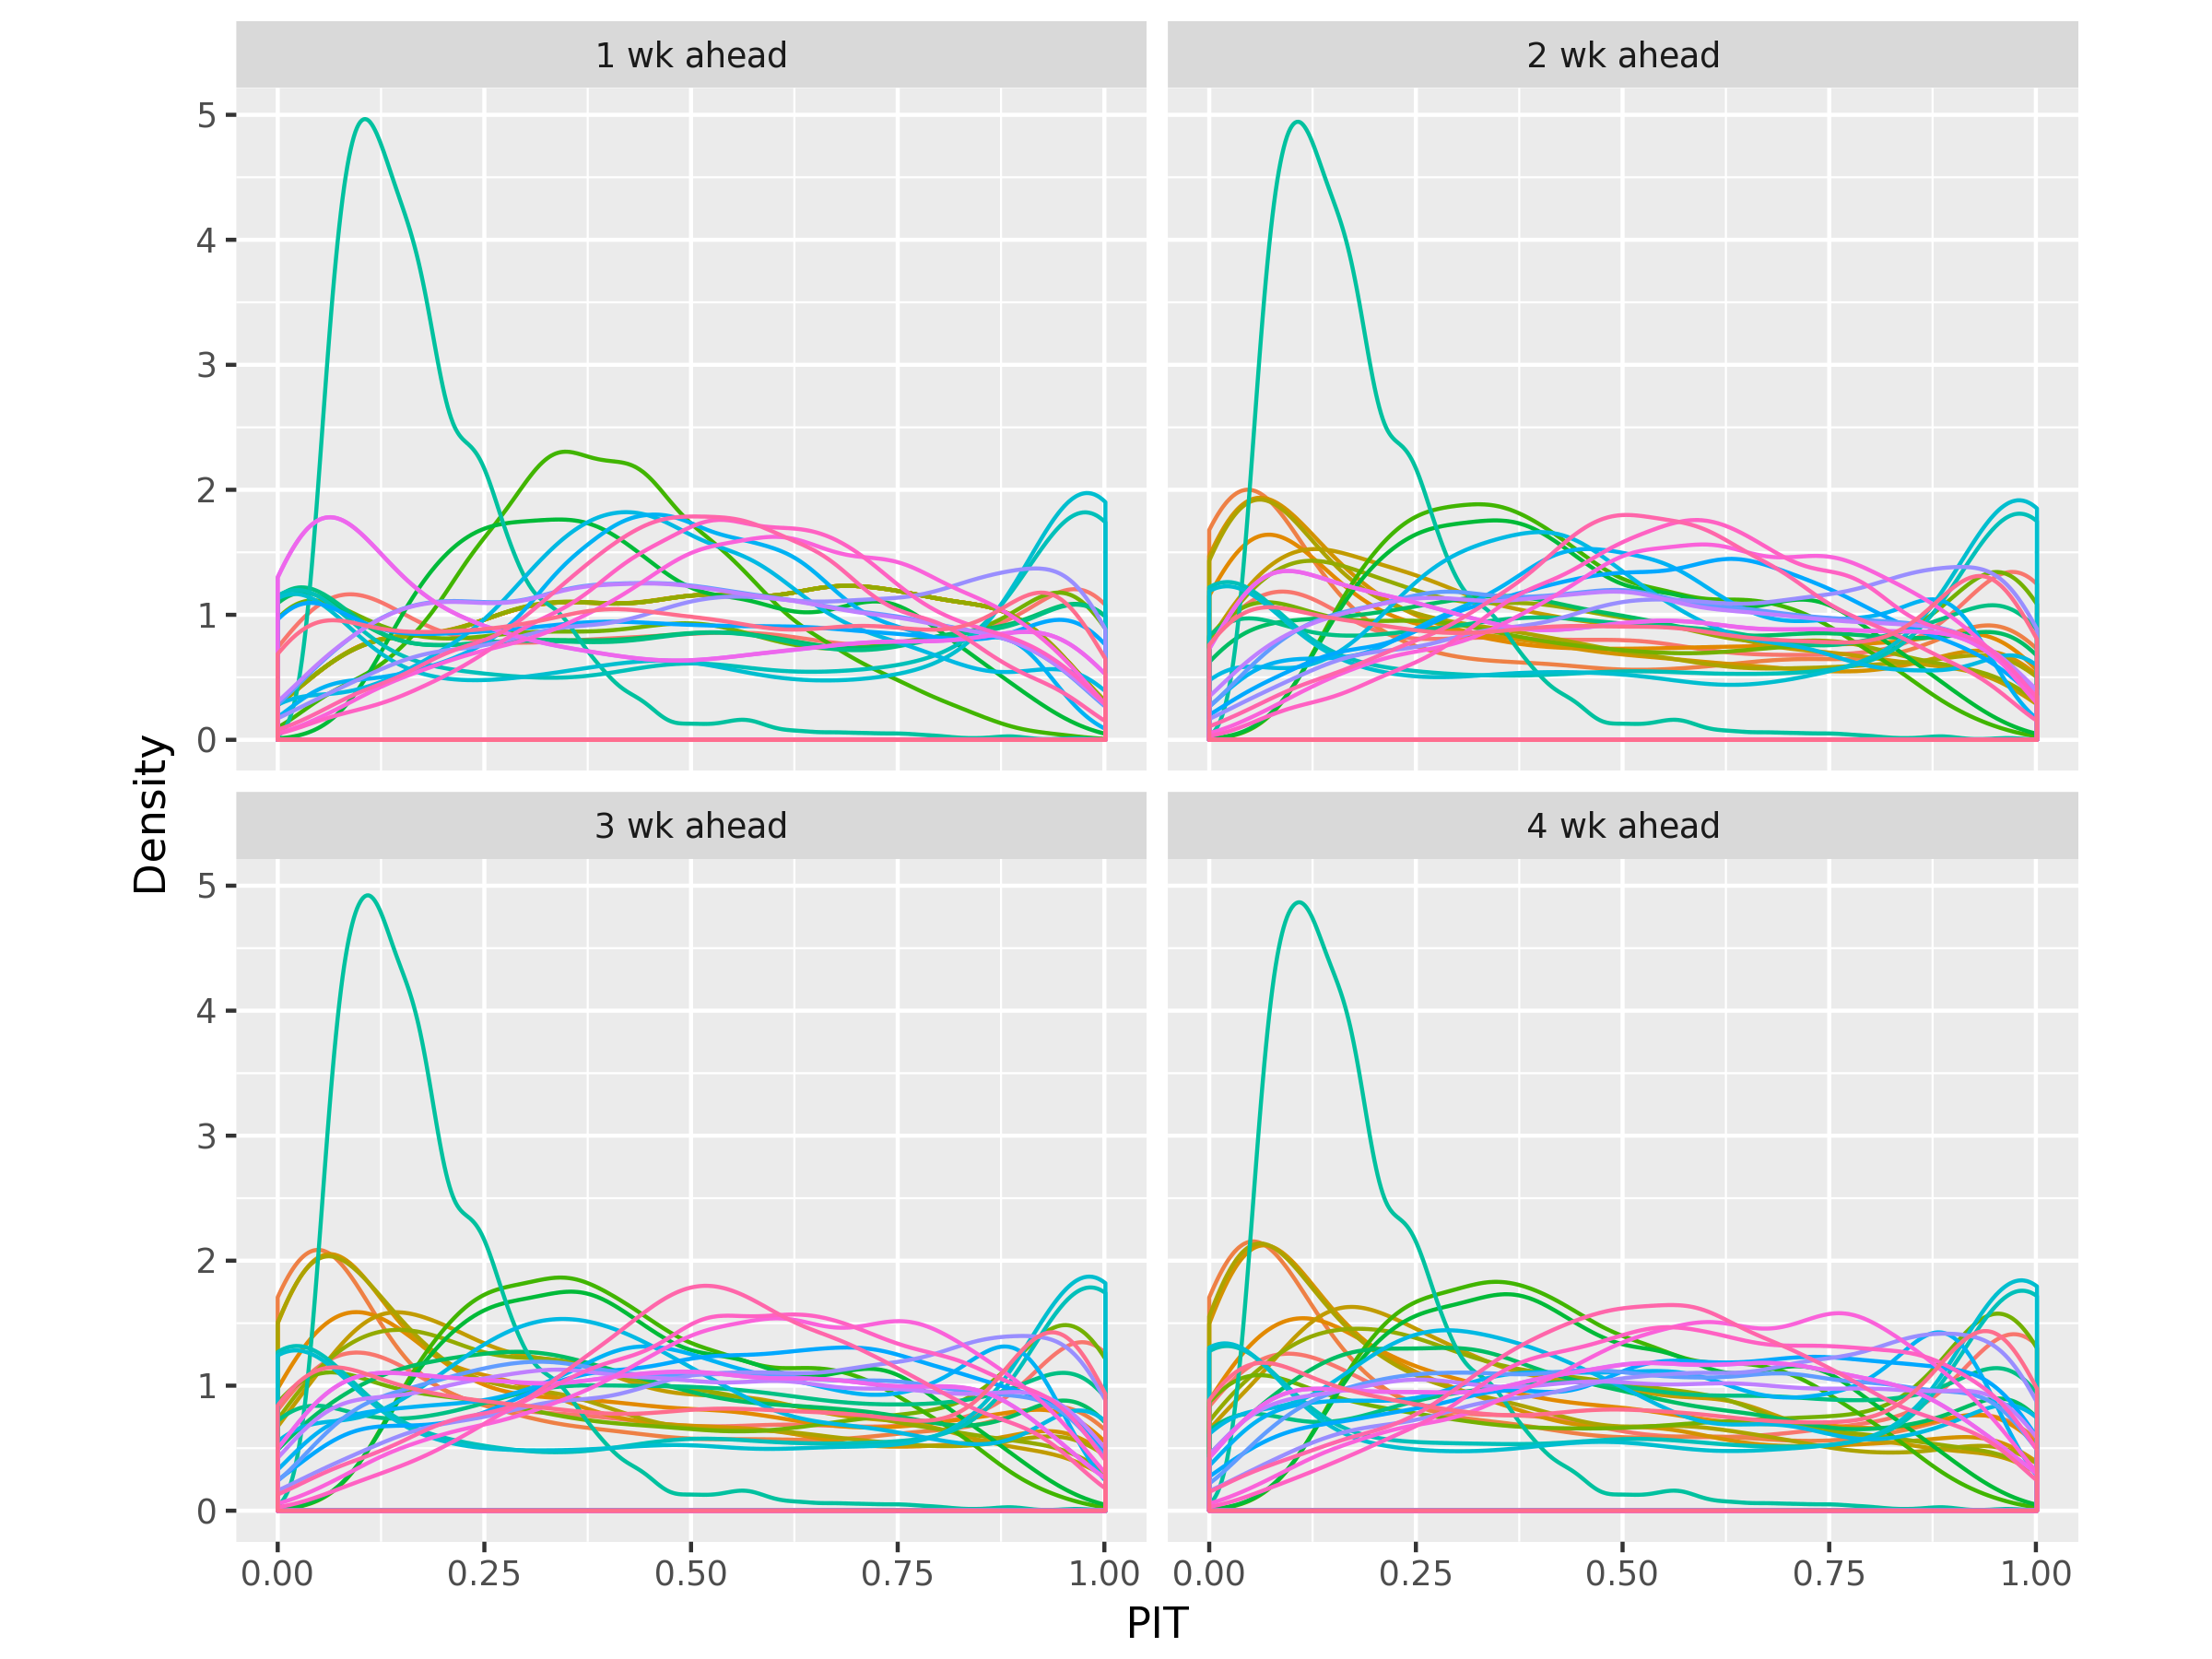
\includegraphics[width=0.85\textwidth]{pit2.png}
\caption{\it Densities of PIT distributions from 27 forecasters submitted to the
  annual FluSight (seasonal influenza forecasting) challenges held by CDC, over
  9 seasons (2010-11 to 2018-19). The PIT densities fall mostly into one of two
  categories: overdispersed with a peak around 0.5, and underdispersed with
  peaks at 0 and 1. (The outlier with a peak at 0.1 is the PIT density of a
  simple baseline forecaster.) Credit: \citet{rumack2022recalibrating}.}           
\label{fig:pit2}
\end{figure}

\subsection{Marginal calibration}

A forecaster with predicted CDF $F$ is said to be \emph{marginally calibrated}
for a target $Y$ if  
\begin{equation}
\label{eq:marginal_calib}
F^{-1}(U) \deq Y,
\end{equation}
where recall $U \sim \mathrm{Unif}(0,1)$. Another way of expressing this is  
\[
\E[F(y)] = \P(Y \leq y), \quad \text{for all $y$},
\]
which is typically how you will see it defined. This also explains its name. 
Interestingly, marginal calibration is \emph{not} the same as probabilistic
calibration, and it is neither more general nor less general. There are
nontrivial forecasters that satisfy \eqref{eq:prob_calib} but not
\eqref{eq:marginal_calib}, and vice versa, to be discussed shortly.  

\paragraph{Dispersion: over and under.}

When $F$ is random and $U \sim \mathrm{Unif}(0,1)$ is independent of $F$, note
that we can then interpret $F^{-1}(U)$ as follows: first draw $F$, then draw a
random variable according to $F$. Thus if $F$ places too much mass on the tails,
then the variance of $F^{-1}(U)$ will be comparably large, and if $F$ places 
insufficient mass in the tails, then the variance of $F^{-1}(U)$ will be
comparably small. This leads to the following definitions, in the context of
marginal calibration:     

\begin{itemize}
\item $F$ is said to be \emph{overdispersed} for $Y$ if $\Var[F^{-1}(U)] > \Var[Y]$;
\item $F$ is said to be \emph{underdispersed} for $Y$ if $\Var[F^{-1}(U)] < \Var[Y]$.
\end{itemize}

\paragraph{PIT versus marginal calibration.}

PIT calibration is a statement about the \emph{joint} distribution of the
forecaster $F$ and target $Y$. Marginal calibration is not; it is only a
statement, as its name suggests, about the \emph{marginal} distributions of $F$
and $Y$. In a sense, it can hence be much simpler to understand and reason about 
than PIT calibration.

To give an example, when we think about systematic miscalibration---a forecaster 
being overdispersed or underdispersed---we might often think about this in terms 
of the forecast distribution being too spread out or too peaked, respectively.
But this intuition is really only justified for marginal calibration, and it is an
incomplete way to think about PIT calibration. This is because the latter is
about how $F$ and $Y$ behave \emph{jointly}. Recall, overdispersion means that
the PIT is too peaked, and underdispersion means that the PIT is too spread
out. This can be entirely due to the dependence between $F$ and $Y$, i.e., it
can happen even when the forecast distribution $F$ is marginally calibrated---it
has ``just enough spread''.

\paragraph{Examples.}

Following \citet{gneiting2007probabilistic}, suppose $\mu$ is drawn from $N(0, 
1)$, and $Y$ is drawn (independently of $\mu$) from $N(\mu, 1)$. Consider (where
we use $F$ to denote both a distribution and a CDF):

\begin{itemize}
\item the \emph{ideal} forecaster: $F = N(\mu, 1)$;
\item the \emph{climatological} forecaster: $F = N(0, 1)$;
\item the \emph{flipped} forecaster: $F = N(-\mu, 1)$;  
\item the \emph{unfocused} forecaster: \smash{$F = \frac{1}{2}[ N(\mu, 1) +
    N(\mu + \tau, 1)]$}, for $\tau = \pm 1$ with equal probability, independent 
  of $Y,\mu$.
\end{itemize}

To gain intuition for the setup, you can think of an underlying sequential
problem, where at time $t$, we draw $\mu_t \sim N(0,1)$, then draw $Y_t \sim
N(\mu_t, 1)$ independently, and the forecasters are $F_t = N(\mu_t, 1)$ (ideal),
$F_t = N(0, 1)$ (climatological), and so on.

Direct calculations, as given in Section 2 of \citet{gneiting2007probabilistic}, 
reveal the following: 

\begin{itemize}
\item the ideal forecaster is both probabilistically and marginally calibrated;  
\item the climatological forecaster is both probalistically and marginally
  calibrated;
\item the flipped forecaster is marginally but not probabilistically
  calibrated; 
\item the unfocused forecaster is probabilistically but not marginally
  calibrated.
\end{itemize}

\subsection{Conditional calibration}

When $Y$ is binary, we can think of a forecaster as providing a predicted
probability $p$ of the event $Y = 1$. In this setting, a forecaster $p$ is said
to be \emph{conditionally calibrated} if
\begin{equation}
\label{eq:cond_calib}
\E[Y|p] = p, \quad \text{almost surely}.  
\end{equation}
This is highly intuitive; for example, when the forecaster outputs a predicted
probability of 0.2, the event $Y=1$ should materialize 20\% of the time, and so
on, for all probability levels. 

Interestingly, and perhaps surprisingly, this is the same as probabilistic
calibration in the binary seting. This is due to \citet{gneiting2013combining}. 

\begin{theorem}
Let $Y$ be binary valued, and suppose a forecaster outputs a predicted
probability $p$ of the event $Y = 1$, with associated predicted CDF 
\[
F(y) = (1-p) \cdot 1\{y \geq 0\} +  p \cdot 1\{y \geq 1\}.
\]
Then $F$ is probabilistically calibrated as in \eqref{eq:prob_calib} if and only
if $p$ is conditionally calibrated as in \eqref{eq:cond_calib}. 
\end{theorem}

\begin{proof}
We prove the ``if'' direction; the ``only if'' direction is less elementary and 
we refer to the proof of Theorem 2.11 in \citet{gneiting2013combining} for
details. Supposing $p$ is probabilistically calibrated, we can write, for $V
\sim \mathrm{Unif}(0,1)$, independent of everything else, 
\[
F^*(Y) = V (1-p) \cdot (1-Y) + (1-p + V p) \cdot Y.
\]
Conditional calibration \eqref{eq:cond_calib} says $Y\,|\,p \sim
\mathrm{Bern}(p)$, and fixing any $t \in [0,1]$, we can compute    
\begin{align*}
\P(F^*(Y) \leq t \,|\, p) 
&= \P\big( V (1-p) (1-Y) + (1-p + V p) Y \leq t \,\big|\, p \big) \\
&= \P\big( V (1-p) \leq t \,\big|\, p \big) \cdot (1-p) + \P\big( V p \leq 
  t-(1-p) \,\big|\, p \big) \cdot p.
\end{align*}
Denoting $a = \P(V (1-p) \leq t \,|\, p)$ and $b = \P(V p \leq t-(1-p) \,|\,
p)$, observe that 
\[
a = \frac{t}{1-p} \wedge 1, 
\quad
b = \frac{t-(1-p)}{p} \vee 0.
\]
Thus when $t \leq 1-p$, we get $\P(F^*(Y) \leq t \,|\, p) = a(1-p) = t$, and
when $t > 1-p$, we get $\P(F^*(Y) \leq t \,|\, p) = (1-p) + bp =
t$. Marginalizing over $p$ proves the probabilistic calibration property
\eqref{eq:prob_calib}.  
\end{proof}

It is also interesting to remark that this equivalence does \emph{not} extend
beyond binary outcomes. For three or more distinct levels of a discrete outcome,
it is no longer true that PIT calibration implies conditional
calibration. \citet{gneiting2022regression} provide a counterexample.  

More broadly, it is worth remarking that the generalization of
\eqref{eq:cond_calib} beyond the binary setting is sometimes called
\emph{auto-calibration}, which requires the predicted CDF $F$ to satisfy  
\begin{equation}  
\label{eq:auto_calib}
Y \,|\, F \deq F^{-1}(U) \,|\, F, \quad \text{almost surely}.   
\end{equation}
A draw from $F^{-1}(U) \,|\, F$ is simply a random variable distributed
according to $F$. Thus, in other words, the property \eqref{eq:auto_calib} says
that almost surely, conditional law of $Y \,|\, F$ should indeed be $F$. You'll 
sometimes see this written as $\cF[Y|F] = F$, almost surely. 

Auto-calibration \eqref{eq:auto_calib} is stronger than all notions of
calibration we have seen thus far, and it implies both probabilistic calibration
\eqref{eq:prob_calib} and marginal calibration
\eqref{eq:marginal_calib}. However, in general, it is not really possible to
check whether auto-calibration holds in practice. See
\citet{gneiting2022regression} for a discussion of this and related topics.

\section{Probability versus quantile aggregation}
\label{sec:prob_quant}

Model aggregation is a rich and important topic in it of itself, and could
easily be the topic of its own lecture. To give a broader context, model
aggregation methods---also called ensemble methods---occupy a central place in
machine learning, both in theory and in practice. Seminal work on this topic
arose in the 1990s, with the development of Bayesian model averaging, bagging,
boosting, and stacking. The machine learning literature has mostly focused on
ensembling point predictions, while ensembling distributions have a had an even 
longer tradition in probabilistic forecasting, dating back to the 1960s. Over
the next two sections, we'll focus on a particularly simple class of aggregation 
methods, linear ones, from the perspective of probabilistic forecasting. The
current section is adapted from Section 3 of  \citet{fakoor2021flexible}.

For convenience, we'll use the term \emph{average} to refer to a weighted linear
combination where the weights are nonnegative and sum to 1. For each
$j=1,\dots,p$, let $F_j$ be a cumulative distribution function (CDF), assumed
continuous, and let $f_j=F_j'$ be its probability density function; let
\smash{$Q_j = F^{-1}_j$} denote the corresponding quantile function, also
assumed continuous, and let $q_j=Q_j'$ the quantile density function. A standard
fact that relates these 
objects:    
\begin{equation}
\label{eq:prob_quant}
q_j(t) = \frac{1}{f_j(Q_j(t))} \quad \text{and} \quad 
f_j(x) = \frac{1}{q_j(F_j(x))}.  
\end{equation}
The first fact can be checked by differentiating $Q_j(F_j(x)) = x$, applying the
chain rule, and reparametrizing via $t=F_j(x)$. The second follows similarly via
$F_j(Q_j(t)) = t$.

\subsection{Two ways of averaging}

We compare and contrast two ways of averaging distributions. The first way is in
probability space, where we define for weights $w_j \geq 0$, $j=1,\dots,p$ such
that \smash{$\sum_{j=1}^p w_j = 1$}, 
\[
F = \sum_{j=1}^p w_j F_j.
\]
The associated density is simply \smash{$f = \sum_{j=1}^p w_j f_j$} since
differentiation is a linear operator. The second way to average is in quantile
space, defining 
\[ 
\bar{Q} = \sum_{j=1}^p w_j Q_j,
\]
where now $\bar{q} = \sum_{j=1}^p w_j q_j$ is the associated quantile density,
again by linearity of differentiation. Denote the CDF and probability density
associated with the quantile average by \smash{$\bar{F} = \bar{Q}^{-1}$}, and
\smash{$\bar{f} = \bar{F}'$}. Note that from \eqref{eq:prob_quant}, we can
reason that \smash{$\bar{f}$} is highly \emph{nonlinear} as a function of $f_j$, 
$j=1,\dots,p$.

A simple example can go a long way to illustrate the differences between the
distributions resulting from probability and quantile averaging. In Figure
\ref{fig:prob_quant}, we compare these two ways of averaging on a pair of
normal distributions with different means and variances.  Here we see that
probability averaging produces the familiar mixture of normals, which is
bimodal. The result of quantile averaging is very different: it is always
unimodal, and instead of interpolating between the tail behaviors of $f_1$ and
$f_2$ (as $f$ does), it appears that \emph{both} tails of \smash{$\bar{f}$} are 
generally thinner than those of $f_1$ and $f_2$.

\begin{figure}[htb]
\centering
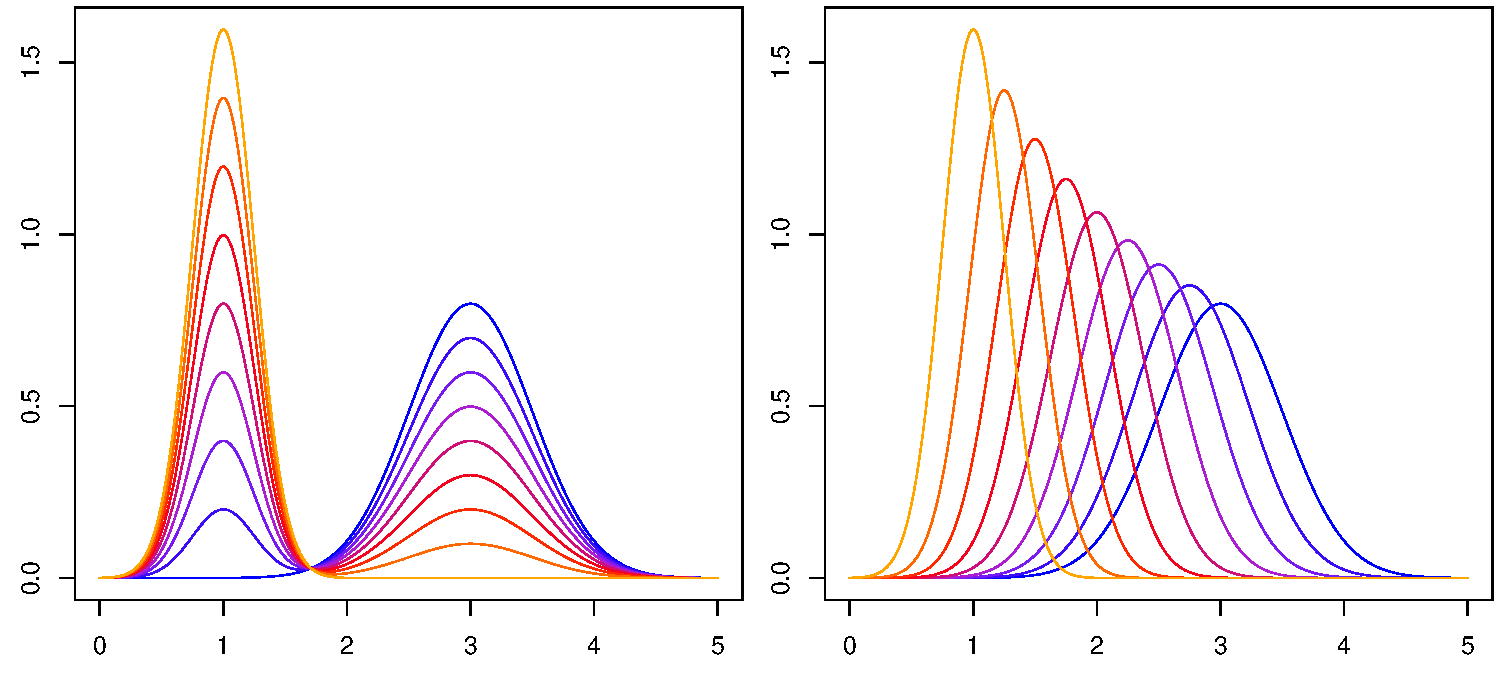
\includegraphics[width=0.9\textwidth]{prob_quant.pdf} 
\caption{\it Densities that result from a probability average (left) or quantile
  average (right) of two normal distributions $N(1,0.25^2)$ and $N(3, 0.5^2)$,
  as the weight on the first density varies from 1 (drawn in orange) to 0
  (drawn in blue). Credit: citet{fakoor2021flexible}.}  
\label{fig:prob_quant}
\end{figure}

It seems that quantile averaging is doing something that is both like
translation and scaling in probability density space. Next we explain this
phenomenon precisely by recalling a classic result.   

\subsection{Shape preservation}

An aggregation procedure $H$ is said to be \emph{shape-preserving} if, for any
location-scale family $\cP$ (such as Normal, t, Laplace, or Cauchy) whose
elements differ only by scale and location parameters, we have     
\[ 
F_j \in \cP, \, j=1,\dots,p \implies F = H(F_1,\dots,F_p) \in \cP.  
\]
Probability averaging is clearly not shape-preserving, however, interestingly,
quantile averaging is: if each $F_j$ a member of the same location-scale family
with a base CDF $L$, then we can write 
\[
F_j(x) = L((x-\theta_j)/\sigma_j),
\]
thus
\[
Q_j(t) = \theta_j + \sigma_j L^{-1}(t),
\]
so \smash{$\bar{Q}$} is still of the form $\theta + \sigma L^{-1}$ and
\smash{$\bar{F}$} is also in the location-scale family. The next proposition
collects this and related results from the literature, due to
\citet{thomas1980appropriate, genest1992vincentization}.  

\begin{proposition}
\label{prop:shape_preservation} \hfill 
\begin{itemize}
\item[(i)] Quantile averaging is shape-preserving.        
\item[(ii)] Location-scale families $\cP$ are the only ones with respect to
  which quantile averaging is a closed operation (meaning $F_j \in \cP$,
  $j=1,\dots,p$ implies \smash{$\bar{F} \in \cP$}).     
\item[(iii)] Quantile averaging is the only aggregation method $H$, of those 
  satisfying (for $h$ not depending on $t$):  
  \[
    H(F_1,\dots,F_p)^{-1}(t) = h(Q_1(t),\dots,Q_p(t)),
  \]
  that is shape-preserving.
\end{itemize}
\end{proposition}

The parts of Proposition \ref{prop:shape_preservation}, taken together, suggest
that quantile averaging is somehow ``tailor-made'' for shape preservation in a
location-scale family---which can be seen as either a pro or a con, depending on
the application one has in mind. To elaborate, suppose that in a quantile
regression ensembling application, each base model outputs a normal distribution
for its predicted distribution at each $x$ (with different means and
variances). If the normal assumption is warranted (i.e., it actually describes
the data generating distribution) then we would want our ensemble to retain 
normality, and quantile averaging would do exactly this. But if the normal
assumption is used only as a working model, and we are looking to combine base
predictions as a way to construct some flexible and robust model, then the
shape-preserving property of quantile averaging would be problematic. In
general, to model arbitrary distributions without imposing strong assumptions,
we are therefore driven to use linear combinations of quantiles that allow 
\emph{different aggregation weights to be used for different quantile levels}, 
of the form \smash{$\bar{Q}(t) = \sum_{j=1}^p w_j(t) Q_j(t)$}. 

\subsection{Moments and sharpness}

Next, we consider moments of the distributions returned by probability and
quantile averages, recalling a result due to \citet{lichtendahl2013better}. For
a distribution $G$, we denote its uncentered moment of order $k \geq 1$ by 
\smash{$m_k(G) = \E_{X \sim G}[X^k]$}.  

\begin{proposition}
\label{prop:moments_sharpness} \hfill
\begin{itemize}
\item[(i)] A probability and quantile average always have equal means:
  \smash{$m_1(F) = m_1(\bar{F})$}.  
\item[(ii)] A quantile average is always sharper than a probability average:
  \smash{$m_k(\bar{F}) \leq m_k(F)$} for any even $k \geq 2$.   
\end{itemize}
\end{proposition}

Note that sharpness is only a desirable property if it does not come at the
expense of calibration. With this in mind, the above result cannot be understood
as a pro or con of quantile averaging without any context on calibration---this
will be studied in Section \ref{sec:aggr_calib}. That said, the relative
sharpness of quantile averages to probability averages is an important general
phenomenon to be aware of.  

\subsection{Tail behavior}

Lastly, we study the action of quantile averaging on the tails of the subsequent
probability density. Simply starting from \smash{$\bar{q} = \sum_{j=1}^p w_j
  q_j$}, differentiating, and using \eqref{eq:prob_quant}, we get
\[
\frac{1}{\bar{f}(\bar{Q}(t))} = \sum_{j=1}^p \frac{w_j}{f_j(Q_j(t))}. 
\]
That is, the probability density \smash{$\bar{f}$} at the level $t$ quantile is
a (weighted) \emph{harmonic mean} of the densities $f_j$ at their respective
level $t$ quantiles. Since harmonic means are generally (much) smaller than
arithmetic means, we would thus expect \smash{$\bar{f}$} to have thinner tails
than $f$. The next result formalizes this. We use $g(x) = o(h(x))$ to mean
$g(x)/h(x) \to 0$ as $x \to \infty$, and $g(x) \asymp h(x)$ to mean $g(x)/h(x)
\to c \in (0, \infty)$ as $x \to \infty$.

\begin{proposition}
\label{prop:tail_behavior}
Assume that $p=2$, $f_2(x) = o(f_1(x))$, and the weights $w_1,w_2$ are
nontrivial (they lie strictly between 0 and 1). Then the density from
probability averaging satisfies $f(v) \asymp f_1(v)$. Assuming further that
$f_1$ is log-concave, the density from quantile averaging satisfies
\smash{$\bar{f}(v) = o(f_1(v))$}.  
\end{proposition}

This result is due to \citet{fakoor2021flexible}. The assumption that $f_1$ is
log-concave for the quantile averaging result is stronger than it needs to be
(as is the restriction to $p=2$), but is used to simplify the proof. 

Proposition \ref{prop:tail_behavior} reiterates the importance of allowing for
level-dependent weights in a linear combination of quantiles. For applications
in which there is considerable uncertainty about extreme events (especially ones
in which there is disagreement in the degree of uncertainty between individual
base models), we would not want an ensemble to de facto inherit a particular
tail behavior---whether thin or thick---but want to endow the aggregation
procedure with the ability to adapt its tail behavior as needed.

\section{Aggregation and (mis)calibration}
\label{sec:aggr_calib}

In this last section, we cover results on the way linear aggregation rules
affect calibration. The setup is as follows. We are given forecasters in the
form of predicted CDFs or predicted quantile functions. We assume that each
forecaster is calibrated, by some definition. We then take an average of CDFs or
quantile functions, and ask whether the result is calibrated, or not.

The results are summarized in Table \ref{tab:aggr_calib}. In a sense, they are
surprising---linear aggregation rules are quite common and popular in practice,
and so the fact that they can destroy PIT calibration in the case of a probability 
average, or marginal calibration in the case of a quantile average, is fairly
disturbing. On the other hand, their proofs are very simple, as we will see in
the following subsections, and arguably these results are not too unexpected, at
least in hindsight. 

\begin{table}[htb]
\centering
\begin{tabular}{c|c|c}
& PIT calibration & Marginal calibration \\
\hline
Probability average & Overdispersed & Calibrated \\
\hline
Quantile average & ? & Underdispersed 
\end{tabular}
\label{tab:aggr_calib}
\caption{\it Summary of known results on aggregation and calibration. In the
  first column, each forecaster is assumed to be PIT calibrated, and in the
  second column, each is assumed to be marginally calibrated. The result in the
  bottom left entry, on the general behavior of a quantile average of PIT
  calibrated forecasters, is currently unknown.} 
\end{table}

\subsection{PIT calibration, probability average}

We start with the assumption that each forecaster is PIT calibrated, in the
sense of \eqref{eq:prob_calib}, and inspect their probability average. The next
result is essentially due to \citet{ranjan2010combining}.  

\begin{theorem}
\label{thm:prob_prob}
Let $F_j$, $j=1,\dots,p$ be CDF forecasts for some target random variable $Y$,
and for fixed weights $w_j \geq 0$, $j=1,\dots,p$, such that
\smash{$\sum_{j=1}^p w_j = 1$}, consider  
\[
F = \sum_{j=1}^p w_j F_j.
\]
Assume that for some $i \not= j$, we have $F_i \not= F_j$ with positive 
probability, and $w_iw_j > 0$. 

\begin{enumerate}[label=\alph*.]
\item For any convex function $\varphi$, it holds that
\[
\E[\varphi(F^*(Y))] \leq \sum_{j=1}^p w_j \E[\varphi(F_j^*(Y))], 
\]
with strict inequality when $\varphi$ is strictly convex.

\item As a result, any of moment $F^*(Y)$ is strictly smaller than the maximum
  corresponding moments of $F_j^*(Y)$, $j=1,\dots,p$. Further, if each
  $F_j^*(Y)$ has the same mean, then the same is true of the central moments.         

\item In particular, if $F_j$, $j=1,\dots,p$ are each probabilistically
  calibrated, as in \eqref{eq:prob_calib}, then $F$ is overdispersed, meaning
  that $\Var(F^*(Y)) < \Var(U)$, where $U \sim \mathrm{Unif}(0,1)$.  
\end{enumerate}
\end{theorem}

\begin{proof}
A key realization to begin is that
\[
F^*(Y) = \sum_{j=1}^p w_j F_j^*(Y),
\]
which we can see by noting that $F$ inherits the left-discontinuities of $F_j$,
$j=1,\dots,p$. For part a, we simply calculate for any convex $\varphi$,  
\[
\E\bigg[\varphi\bigg( \sum_{j=1}^p w_j F_j^*(Y) \bigg)\bigg] \leq 
\sum_{j=1}^p w_j \E[\varphi(F_j^*(Y))],
\]
by Jensen's inequality, with strict inequality when $\varphi$ is strictly 
convex (by our assumption about the existence of a pair $F_i,F_j$ that are 
not equal with positive probability, and $w_iw_j>0$).

The first statement in part b is simply proved by considering $\varphi(x) = x^k$
for any positive integer $k$. In the case that $F_j^*(Y)$, $j=1,\dots,p$ all
have the same mean, note that by taking $\varphi(x) = \pm x$, we learn that
$F^*(Y)$ must also have the same mean, which proves the second statement in part
b about central moments.

Lastly, part c is just the special case for the variance, i.e., second central
moment, when each $F_j^*(Y) \sim \mathrm{Unif}(0,1)$, $j=1,\dots,p$.
\end{proof}

The fact that any linear combination of probabilistically calibrated CDF
forecasters must be miscalibrated and systematically overdispersed (part c) is
simple but striking. In the binary case, where $Y \in \{0,1\}$, the same is true
when we replace the notion of probabilistic calibration with conditional
calibration (recalling the equivalence between the two), which reproduces an
earlier result from \citet{ranjan2010combining}.  

\subsection{Marginal calibration, probability average}

Now we move to the case where each forecaster is PIT calibrated, and still
consider a probability average. The next result is very simple but 
noting, and once again emphasizes the differences between marginal and
probabilistic calibration. 

\begin{theorem}
\label{thm:marginal_prob}
Let $F_j$, $j=1,\dots,p$ be CDF forecasts for some target random variable $Y$,
and for fixed weights $w_j \geq 0$, $j=1,\dots,p$, such that
\smash{$\sum_{j=1}^p w_j = 1$}, consider  
\[
F = \sum_{j=1}^p w_j F_j.
\]
If $F_j$, $j=1,\dots,p$ are each marginally calibrated, as in
\eqref{eq:marginal_calib}, then $F$ is also marginally calibrated.  
\end{theorem}

\begin{proof}
We simply compute 
\[
\E\bigg[ \sum_{j=1}^p w_j F_j(y) \bigg] = \sum_{j=1}^p w_j \P(Y \leq y) =  
\P(Y \leq y). 
\]
\end{proof}

\subsection{Marginal calibration, quantile average}

Keeping marginal calibration in mind, but moving to a quantile average (hence
moving clockwise through the results in Table \ref{tab:aggr_calib}), we have the
following result. 

\begin{theorem}
\label{thm:marginal_quant}
Let $F_j^{-1}$, $j=1,\dots,p$ be quantile forecasts for some target random
variable $Y$, and for fixed weights $w_j \geq 0$, $j=1,\dots,p$, such that
\smash{$\sum_{j=1}^p w_j = 1$}, consider   
\[
F^{-1} = \sum_{j=1}^p w_j F_j^{-1}.
\]
Assume that for some $i \not= j$, we have $F_i^{-1} \not= F_j^{-1}$ with
positive probability, and $w_iw_j > 0$. 

\begin{enumerate}[label=\alph*.]
\item For any convex function $\varphi$, and $U \sim \mathrm{Unif}(0,1)$ it
  holds that 
\[
\E[\varphi(F^{-1}(U))] \leq \sum_{j=1}^p w_j \E[\varphi(F_j^{-1}(U))], 
\]
with strict inequality when $\varphi$ is strictly convex.

\item As a result, any of moment $F^{-1}(U)$ is strictly smaller than the
  maximum corresponding moments of $F_j^{-1}(U)$, $j=1,\dots,p$. Further, if each 
  $F_j^{-1}(U)$ has the same mean, then the same is true of the central moments.      

\item In particular, if $F_j$, $j=1,\dots,p$ are each marginally calibrated, as
  in \eqref{eq:marginal_calib}, then $F$ is underdispersed, meaning 
  that $\Var(F^{-1}(U)) < \Var(Y)$.
\end{enumerate}
\end{theorem}

\begin{proof}
The proof is similar to that of Theorem \ref{thm:prob_prob}. For part a, we
calculate for any convex $\varphi$,   
\[
\E[\varphi(F^{-1}(U))] \leq \sum_{j=1}^p \E[\varphi(F_j^{-1}(U))],
\]
by Jensen's inequality, with strict inequality when $\varphi$ is strictly 
convex (again by our assumption about the existence of a pair
$F_i^{-1},F_j^{-1}$ that are not equal with positive probability, and
$w_iw_j>0$). The rest of the proof is identical to that of Theorem
\ref{thm:prob_prob}.  
\end{proof}

Again, the fact that any linear combination of marginally calibrated quantile
forecasters must be miscalibrated and systematically underdispersed (part c) is
simple but striking.

\subsection{PIT calibration, quantile average}

This case seems to elude simple analysis (at least for now). If the world was
just, then one might hope (by symmetry in Table \ref{tab:aggr_calib}) that a
quantile average of PIT calibrated forecasters would itself be calibrated.
However, this is not the case, because---sadly---we know of at least one case
where it can be shown analytically that the quantile average here is
overdispersed.   

Given what we know about the relationship between probability and quantile
averages though (recall, e.g., Proposition \ref{prop:moments_sharpness}), one 
might still hope that a quantile average is \emph{less} overdispersed than the
corresponding probability average, when the constituent forecasters are all PIT 
calibrated. 

\bibliographystyle{plainnat}
\bibliography{../../common/ryantibs}

\end{document}
